\documentclass[tikz,border=7pt]{standalone}
\usepackage[T1]{fontenc}
\usepackage{lmodern}
\usetikzlibrary{arrows.meta,positioning,fit,calc}

\definecolor{inputblue}{HTML}{E7F0FA}
\definecolor{encoderpurple}{HTML}{EEE8FA}
\definecolor{tokengold}{HTML}{FFF2CE}
\definecolor{fusiongreen}{HTML}{E6F3EE}
\definecolor{latentorange}{HTML}{FFF0E5}
\definecolor{decoderrose}{HTML}{FBE6EF}
\definecolor{notegray}{HTML}{F2F4F6}
\definecolor{ink}{HTML}{29333D}

\tikzset{
  block/.style={
    draw=ink,
    rounded corners=2.4pt,
    line width=0.72pt,
    align=center,
    inner sep=6pt,
    font=\sffamily\small,
    minimum height=18mm
  },
  smallblock/.style={
    block,
    font=\sffamily\footnotesize,
    minimum height=10.5mm
  },
  bottleneck/.style={
    draw=ink,
    rounded corners=2.4pt,
    line width=0.72pt,
    align=center,
    inner sep=4pt,
    font=\sffamily\small,
    minimum height=12mm
  },
  group/.style={
    draw=ink,
    rounded corners=3pt,
    line width=0.58pt,
    dashed,
    inner sep=6pt
  },
  arrow/.style={
    -{Stealth[length=2.2mm,width=1.8mm]},
    draw=ink,
    line width=0.78pt
  },
  note/.style={
    draw=ink,
    rounded corners=2pt,
    fill=notegray,
    align=center,
    inner sep=5pt,
    font=\sffamily\footnotesize,
    minimum height=10mm
  }
}

\begin{document}
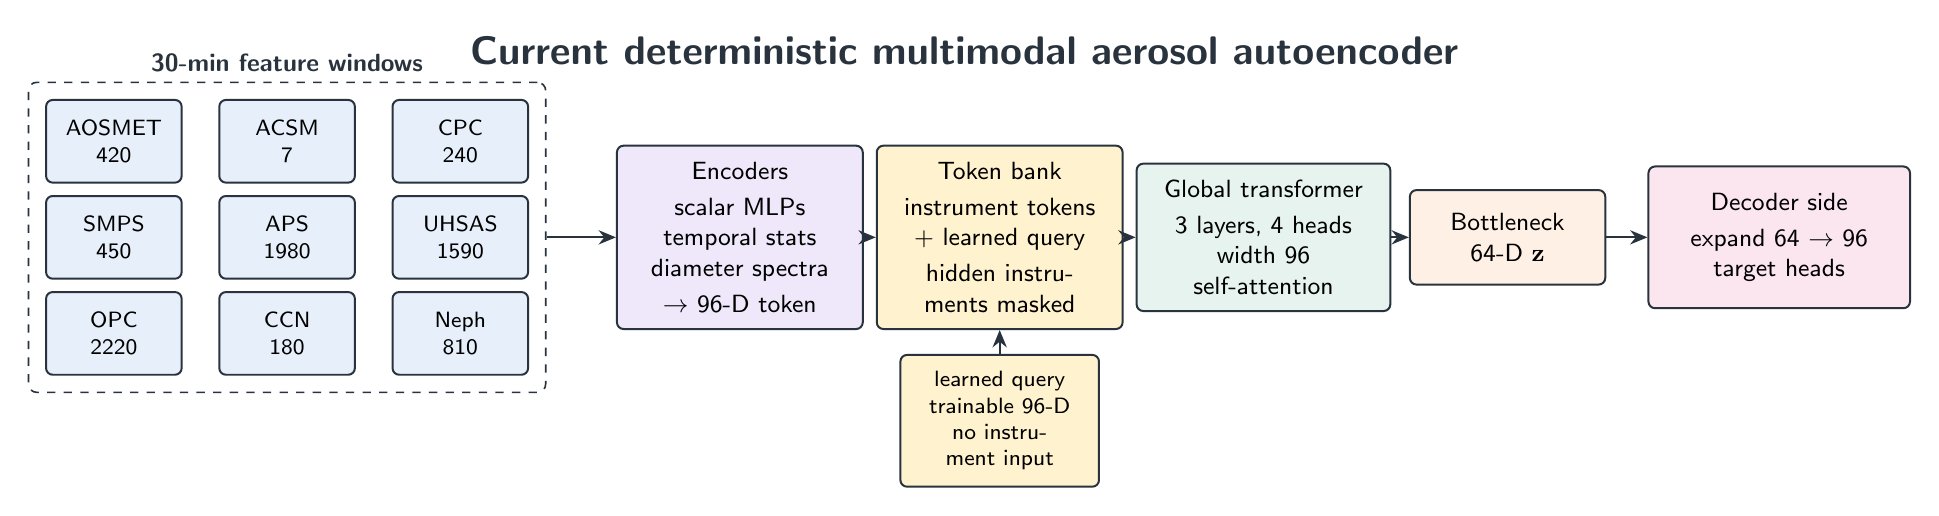
\begin{tikzpicture}[x=1cm,y=1cm]
  \node[font=\sffamily\bfseries\Large, text=ink] at (11.6,6.15)
    {Current deterministic multimodal aerosol autoencoder};

  \node[smallblock, fill=inputblue, text width=13mm] (met) at (0.80,5.00)
    {AOSMET\\420};
  \node[smallblock, fill=inputblue, text width=13mm] (acsm) at (3.00,5.00)
    {ACSM\\7};
  \node[smallblock, fill=inputblue, text width=13mm] (cpc) at (5.20,5.00)
    {CPC\\240};
  \node[smallblock, fill=inputblue, text width=13mm] (smps) at (0.80,3.78)
    {SMPS\\450};
  \node[smallblock, fill=inputblue, text width=13mm] (aps) at (3.00,3.78)
    {APS\\1980};
  \node[smallblock, fill=inputblue, text width=13mm] (uhsas) at (5.20,3.78)
    {UHSAS\\1590};
  \node[smallblock, fill=inputblue, text width=13mm] (opc) at (0.80,2.56)
    {OPC\\2220};
  \node[smallblock, fill=inputblue, text width=13mm] (ccn) at (3.00,2.56)
    {CCN\\180};
  \node[smallblock, fill=inputblue, text width=13mm] (neph) at (5.20,2.56)
    {Neph\\810};
  \node[group, fit=(met)(acsm)(cpc)(smps)(aps)(uhsas)(opc)(ccn)(neph),
    label={[font=\sffamily\bfseries\small,text=ink]above:30-min feature windows}] (inputgroup) {};

  \node[block, fill=encoderpurple, text width=27mm] (enc) at (8.75,3.78)
    {Encoders\\[2pt]
     scalar MLPs\\
     temporal stats\\
     diameter spectra\\[2pt]
     $\rightarrow$ 96-D token};

  \node[block, fill=tokengold, text width=27mm] (tokens) at (12.05,3.78)
    {Token bank\\[2pt]
     instrument tokens\\
     + learned query\\[2pt]
     hidden instruments masked};

  \node[block, fill=fusiongreen, text width=28mm] (xfmr) at (15.40,3.78)
    {Global transformer\\[2pt]
     3 layers, 4 heads\\
     width 96\\
     self-attention};

  \node[bottleneck, fill=latentorange, text width=22mm] (latent) at (18.50,3.78)
    {Bottleneck\\64-D $\mathbf{z}$};

  \node[block, fill=decoderrose, text width=29mm] (decode) at (21.95,3.78)
    {Decoder side\\[2pt]
     expand 64 $\rightarrow$ 96\\
     target heads};

  \draw[arrow] (inputgroup.east) -- (enc.west);
  \draw[arrow] (enc.east) -- (tokens.west);
  \draw[arrow] (tokens.east) -- (xfmr.west);
  \draw[arrow] (xfmr.east) -- (latent.west);
  \draw[arrow] (latent.east) -- (decode.west);

  \node[smallblock, fill=tokengold, text width=21mm] (query) at (12.05,1.45)
    {learned query\\trainable 96-D\\no instrument input};
  \draw[arrow, rounded corners=4pt] (query.north) -- ++(0,0.34) -- (tokens.south);
\end{tikzpicture}
\end{document}
